\subsection{Häufige Parametrisierungen}
    \subsubsection{Ellipse}
    \begin{align*}
        \overrightarrow{r}(t) = \binom{a \cdot cos(t) + x_0}{b \cdot sin(t) + y_0}\\
        \text{Sonderfall Kreis mit Radius } a = b
    \end{align*}
    \begin{center}
        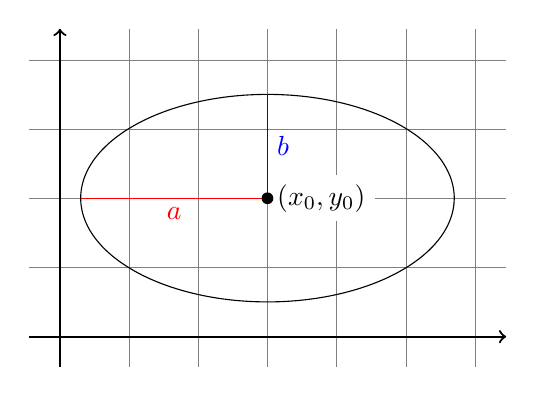
\begin{tikzpicture}[x=0.75pt,y=0.75pt,yscale=-1,xscale=1]
            %coordinatum system
            \foreach \i in {0, ..., 6} {
                \draw [very thin,gray] (\i * 33.33, -15) -- (\i * 33.33, 148);
            }
            \foreach \i in {0, ..., 4} {
                \draw [very thin,gray] (-15 ,\i * 33.33) -- (215 ,\i * 33.33);
            }
            \draw[thick, <-] (0, -15) -- (0, 148);
            \draw[thick, ->] (-15, 133.33) -- (215, 133.33);
            %
            %Ellipse
            \draw plot [smooth, samples = 100, domain = 0:500] ({90 * cos(\x) + 100}, {50 * sin(\x) + 66.6});
            %a
            \draw [red] (100, 66.66) -- (55, 66.66) node[anchor = north, red] {$a$} -- (10, 66.66);
            %b
            \draw [blue] (100, 66.66) -- (100, 41.66) node[anchor = west, blue] {$b$} -- (100, 16.66);
            %Midpoint
            \draw (100, 66.66) node[right, fill=white] {$(x_0, y_0)$} node[circle, fill, inner sep = 1.5pt]{};
        \end{tikzpicture}\\
    \end{center}
    
    \subsubsection{Zykloide}
    \begin{align*}
        \overrightarrow{r}(t) = \binom{rt - a sin(t)}{r - a cos(t)}\\
        \text{Sonderfall Gewöhnliche Zykloide } r = a\\
    \end{align*}

    \subsubsection{Epizykloide}
    \begin{align*}
        \overrightarrow{r}(t) = \binom{R cos(t) - a cos(\frac{R}{r} t)}{R sin(t) - a sin(\frac{R}{r} t)}\\
        \text{Sonderfall Kardioide } R = 2r, r = a\\
    \end{align*}

    \subsubsection{Hypozykloide}
    \begin{align*}
        \overrightarrow{r}(t) = \binom{R cos(t) + a cos(\frac{R}{r} t)}{R sin(t) - a sin(\frac{R}{r} t)}\\
    \end{align*}

    \subsubsection{Lissajous-Figuren}
    \begin{align*}
        \overrightarrow{r}(t) = \binom{a_1 sin(\omega_1 t + \varphi_1)}{a_2 sin(\omega_2 t + \varphi_2)}
    \end{align*}